\documentclass{article}
\usepackage[T1]{fontenc}
\usepackage[utf8]{inputenc}
\usepackage{cs-337}


\begin{document}

\thispagestyle{empty}

\titleBC
\tableofcontents
\clearpage

\setcounter{section}{-1}

\section{Notation and Prerequisites}
	
	Given $n \in \N$, $[n]$ denotes the set $\{1,\ldots,n\}$ and $[n]_0$ denotes the set $[n] \cup \{0\}$.\\
	$S(n,k)$, a Stirling number of the second kind, is the number of partitions of $[n]$ into exactly $k$ parts. $s(n,k)$, a Stirling number of the first kind, is the number of permutations of $[n]$ with exactly $k$ cycles.\\
	
\clearpage
% \section{Introduction}

\begin{exercise}
	Recall that the number of $k$-subsets of $[n]$ is $\binom{n}{k}$. Given a $k$-subset $S = \{x_1,\ldots,x_k\}$ of $[n]$, we write $S_< = \{x_1,\ldots,x_k\}_<$ to denote that $x_1<x_2<\cdots<x_k$. Determine the number of $k$-subsets $\{x_1,\ldots,x_k\}_<$ of $[n]$ such that $x_i \cong i \mod 2$.
\end{exercise}
For example, for $n=6$ and $k=3$, we have the subsets $\{1,4,5\},\{1,2,3\},\{1,2,5\},\{3,4,5\}$.


Broadly, there are three types of ``answers'': a formula, a recurrence, and a generating function. A great example of the second and third is the following.\\
% Euler's Theorem
$p(n)$, the number of number partitions of $n$, is given by the generating function
\[ \sum_{n \ge 0} p(n) x^n = \prod_{i \ge 1} \frac{1}{1-x^i}. \]
Using this, a recursion may be obtained as well.
We do \emph{not} plug in values for $x$ in the above. We merely look at the coefficient of $x^n$ in it. We want the coefficient to be a finite sum for all $n$. If it is an infinite sum, convergence issues may arise.

% www.math.iitb.ac.in/~krishnan/phd-2022/

% The number of derangements of $[n]$ is the integer closest to $n!/e$.
% Bell number B_n (number of set partitions of $[n]$) : \sum_{n \ge 0} B_n x^n / n! = e^{e^x - 1}.

\subsection{Counting in \texorpdfstring{$\mathfrak{S}_n$}{Sn}}

	Recall that $\mathfrak{S}_n$ is generated by transpositions. A transposition $(i,j)$ is a permutation $\sigma$ defined by
	\[ \sigma(k) = \begin{cases} j, & k=i, \\ i, & k=j, \\ k, & \text{otherwise.} \end{cases} \]
	In fact, $\mathfrak{S}_n$ is generated by the set of just ``adjacent transpositions'' $S_i = (i,i+1)$ for $1 \le i < n$.
	We have
	\begin{align*}
		S_i^2 &= \Id \\
		S_i S_{i+1} S_i &= S_{i+1} S_i S_{i+1} \\
		S_i S_j &= S_j S_i \text{ if $|i-j| > 2$.}
	\end{align*}


	\begin{fdef}
		Given a permutation $\pi \in \mathfrak{S}_n$, define the \emph{length} $\ell(\pi)$ of $\pi$ to be the smallest $k$ such that there exist adjacent transpositions $\sigma_1,\cdots,\sigma_k$ such that $\pi = \sigma_1\cdots\sigma_k$.
	\end{fdef}
	% PRESENT PROOF THAT WE CAN WRITE IT IN THIS WAY ON TUESDAY -- 02/08/2022
	% DONE.

	\begin{fprop}
		Consider the \emph{inversion number} $\inv(\pi)$ of a permutation, defined by
		\[ \inv(\pi) = \left|\{ 1 \le i \le j \le n : \pi_i > \pi_j \}\right|. \]
		Then, $\ell(\pi) = \inv(\pi)$.
	\end{fprop}

	\begin{fdef}
		The \emph{sign} of a permutation $\pi$ is defined by $\sign(\pi) = (-1)^{\inv(\pi)}$. Equivalently,
		\[ \sign(\pi) = \frac{\prod_{1 \le i < j \le n} (x_{pi_i} - x_{\pi_j})}{\prod_{1 \le i < j \le n} (x_i - x_j)}. \]
	\end{fdef}

	% LATER, STUDY NUMBER OF ``REDUCED'' PRODUCTS? (NUMBER OF WAYS IN WHICH PI CAN BE WRITTEN AS A PRODUCT OF L(PI) ADJ TRANSPOSITIONS)


	It is straightforward to see that for all $\pi \in \mathfrak{S}_n$, $0 \le \inv(\pi) \le \binom{n}{2}$.
	\begin{fprop}
		\label{prop: inv n}
		Consider $\inv_n(q) = \sum_{\pi \in \mathfrak{S}_n} q^{\inv(\pi)}$. Then,
		\[ \inv_n(q) = \prod_{1 \le m \le n} [n]_q, \]
		where
		\[ [m]_q = \begin{cases} 1 + q + \cdots + q^{m-1}, & m \ge 1, \\ 0, & m = 0. \end{cases} \]
	\end{fprop}
	This quantity $[m]_q$ is called the $q$-analogue of $m$, and similarly, the $q$-analogue of $n!$ is $\prod_{i=1}^n [m]_q$ (this is slightly vague).
	Note in particular that $n! = \inv_n(1)$.
	\begin{proof}
		We prove this by induction. It is easily verified for $n = 2$.\\
		Take $\sigma \in \mathfrak{S}_{n-1}$. There are $n$ ``gaps'' where $n$ can be ``placed'' in $\sigma$ to get a permutation in $\mathfrak{S}_n$. If we place it in the $i$th position from the end (for $0 \le i \le n-1$), the inversion number of the newly obtained permutation is $i$ more than the inversion number of $\sigma$.\\
		As a result,
		\[ \inv_n(q) = \inv_{n-1}(q) + q \inv_{n-1}(q) + q^2 \inv_{n-1}(q) + \cdots + q^{n-1} \inv_{n-1}(q) = [n]_q \inv_{n-1}(q), \]
		where the $q^i \inv_{n-1}(q)$ term corresponds to the case where $n$ is placed in the $i$th position from the end. The required follows by the inductive hypothesis.
	\end{proof}

	\begin{definition}[Descent]
		For $\pi \in \mathfrak{S}_n$, define the \emph{descents} $\DES(\pi) = \{i \in [n-1] : \pi_i > \pi_{i+1}\}$, $\des(\pi) = |\DES(\pi)|$, and $\maj(\pi) = \sum_{i \in \DES(\pi)} i$. 
	\end{definition}
	There are central limit theorems for many of these parameters, which we shall not study.\\
	A permutation $\pi$ has $\des(\pi) + 1$ many ``increasing runs''.

	For example, for the permutation $\pi = (1\mapsto 5,2\mapsto1,3\mapsto2,4\mapsto6,5\mapsto4,6\mapsto3) \in \mathfrak{S}_6$, $\DES(\pi) = \{1,4,5\}$, $\des(\pi) = 3$, and $\maj(\pi) = 10$.

	\begin{fprop}
		\label{prop: maj n}
		The distribution of $\maj(\pi)$ over $\mathfrak{S}_n$ is the same as that of $\inv(\pi)$. Equivalently,
		\[ \maj_n(q) = \sum_{\pi \in \mathfrak{S}_n} q^{\maj(\pi)} = \prod_{m=1}^n [m]_q = \inv_n(q). \] 
	\end{fprop}
	This result took nearly 50 years to prove!
	\begin{proof}
		The strategy is similar to that of \Cref{prop: inv n}. Let $\pi \in \mathfrak{S}_{n-1}$. As before, there are $n$ positions to insert $n$.
		% An insertion increases $\maj$ (compared to $\pi$) only if it is placed in the middle of an increasing run. That is, we must place it  Further, in this case, it increases $\des$ by $1$. What is the sum of $\maj$ increases over all possible insertions? 
		\begin{itemize}
			\item Label the positions of descents of $\sigma$ and the last position from right ot left as $0,1,\ldots,\des(\pi)$.
			\item Label the remaining positions from left to right as $\des(\pi)+1,\ldots,n-1$.
		\end{itemize}
		We claim that inserting $n$ at a position increases $\maj$ by the labelled amount.\\
		If inserted anywhere, all the descent positions starting from there increase by $1$. This explains why the increase is equal to the labelled quantity for positions that are descents, since no new descents are introduced. In the case where we insert it in a position of non-descent, we further introduce a new descent at the position of insertion of $n$, which explains why the increase is equal tot he labelled quantity for positions that are not descents.\\
		The remainder of the proof is identical to that of \Cref{prop: inv n}, since the increases are in bijection with $[n-1]_0$.
	\end{proof}

	\begin{definition}
		A parameter $f : \mathfrak{S}_n \to \R$ of permutations such that
		\[ \sum_{\pi \in \mathfrak{S}_n} q^{f(\pi)} = \prod_{1 \le m \le n} [m]_q \]
		is said to be \emph{Mahonian}.
	\end{definition}

	As we saw in \Cref{prop: inv n,prop: maj n}, both $\inv$ and $\maj$ are Mahonian.

\subsection{Counting spanning trees}

	\begin{problem*}
		Count the number of spanning trees in an arbitrary (finite) graph $G$.
	\end{problem*}

	This was solved by Kirchhoff using the Matrix Tree Theorem.
	
	\begin{ftheo}[Matrix Tree Theorem]
		Consider the \emph{Laplacian} $L = D-A$ of a graph $G$, where $A$ is its adjacency matrix and $D$ is a diagonal matrix with the diagonal entries being the degrees of the vertices. The determinant of any $(n-1)\times(n-1)$ submatrix of $L$ obtained by omitting any arbirary row and column is equal to the number of spanning trees of $G$.
	\end{ftheo}

	% oriented incidence matrix is totally unimodular -- poincare

	In particular, when $G = K_n$, we end up getting the following.

	\begin{ftheo}[Cayley's Theorem]
		\label{theo: cayleys theorem}
		The number of spanningtrees in $K_n$ is $n^{n-2}$.
	\end{ftheo}
	One proof by Pr\"{u}fer gives an explicit bijection between spanning trees and sequences $(v_1,\ldots,v_{n-2})$ of vertices in $G$.\\
	Another proof is of course using the matrix tree theorem, which reduces it to a simple determinant calculation.\\
	Joyal gave another bijection between elements of the form $(T,u,v)$ where $T$ is a spanning tree and $u,v$ are vertices in $G$, and functions from $[n] \to [n]$.\\

	The proof we give uses exponential generating functions. Recall the following result, which we give without proof. Interested readers may consult Corollary 5.1.6 of \cite{ec2} for further details.

	\begin{ftheo}[Exponential Formula]
		\label{ec2: egf sum over partitions}
		Let $\{f_n\}$ be a sequence with exponential generating function
		\[ F(x) = \sum_{n \ge 1} f_n \frac{x^n}{n!}. \]
		Define the sequence $h_n$ by
		\[ h_n = \sum_{\substack{\pi \in \operatorname{SetPartn}([n]) \\ \pi = \{S_1,\ldots,S_k\}}} f_{|S_1|} f_{|S_2|} \cdots f_{|S_k|}  \]
		and $h_0 = 1$, and let
		\[ H(x) = \sum_{n \ge 0} h_n \frac{x^n}{n!}. \]
		Then,
		\[ H(x) = \exp(F(x)) \]
	\end{ftheo}
	Note that the summation of $F$ is for $n \ge 1$, because we may assume that $f_0 = 0$ since $f_0$ does not appear in the expression of any $h_n$.\\

	\begin{fdef}[Compositional inverse]
		Generating functions $F$ and $G$ are said to be \emph{compositional inverses} (of each other) if $F(G(x)) = G(F(x)) = x$.
	\end{fdef}

	Let
	\[ F(x) = \sum_{n \ge 0} f_n x^n \text{ and } G(x) = \sum_{n \ge 0} g_n x^n \]
	be compositional inverses of each other. It is reasonably straightforward to show that $f_0 = g_0 = 0$ and $f_1,g_1 \ne 0$. The first condition implies that the coefficient of any $x^n$ in $F\circ G$ (or $G \circ F$) is finite. 

	\begin{ftheo}[Lagrange Inversion Theorem]
		\label{theo: lagrange inversion}
		Let
		\[ F(x) = \sum_{n \ge 0} f_n x^n \text{ and } G(x) = \sum_{n \ge 0} g_n x^n \]
		be compositional inverses of each other. Then, $ng_n$ is the coefficient of $1/x$ in $(1/F(x))^n$.
	\end{ftheo}
	Equivalently, $ng_n$ is the coefficient of $x^{n-1}$ in $(x/F(x))^n$.
	\begin{proof}
		We have
		\[ x = G(F(x)) = \sum_{i \ge 0} g_i F(x)^i. \]
		Differentiating,
		\[ 1 = \sum_{i \ge 0} g_i i F(x)^{i-1} F'(x). \]
		As a result,
		\[ \left(\frac{1}{F(x)}\right)^n = \sum_{i \ge 0} g_i i F(x)^{i-1-n} F'(x).  \]
		Whenever $i \ne n$, the coefficient of $1/x$ in $F(x)^{i-1-n} F'(x) = \left(F(x)^{i-n}/(i-n)\right)'$ is zero. Indeed, recall that the coefficient of $1/x$ in the derivative of any power series with possibly negative exponents is zero.\\
		As a result, the coefficient of $1/x$ in $(1/F(x))^n$ is equal to the coefficient of $1/x$ in $g_n n F'(x) / F(x)$.
		% , which is the constant term in $n g_n x F'(x) / F(x)$ -- observe that there cannot be a $x^{-m}$ term for any $m \ge 2$.
		We have
		\[ \frac{F'(x)}{F(x)} = \frac{f_1 + 2f_2x + \cdots}{f_1x + f_2x^2 + \cdots}. \]
		The constant term in this is $f_1/f_1 = 1$, and the desideratum follows. 
	\end{proof}

	At long last, let us return to \nameref{theo: cayleys theorem}.

	\begin{proof}[Proof of \nameref{theo: cayleys theorem}]
		Instead of looking at the number $\text{T}_n$ of spanning trees, we shall look at $\text{RT}_n$, the number of \emph{rooted} spanning trees. Clearly, $\text{RT}_n = n \text{T}_n$.\\
		Define $\text{RF}_n$ to be the number of rooted forests on $[n]$ and let
		\begin{align*}
			\operatorname{RF}(x) &= \sum_{n \ge 0} \text{RF}_n \frac{x^n}{n!} \\
			\operatorname{RT}(x) &= \sum_{n \ge 0} \text{RT}_n \frac{x^n}{n!}.
		\end{align*}

		Using \Cref{ec2: egf sum over partitions}, it is not too difficult to see that
		\begin{equation}
			\label{eqn 1}
			\operatorname{RF}(x) = \exp(\operatorname{RT}(x)).
		\end{equation}

		\textbf{Claim} (Polya). $\text{RT}_{n+1} = (n+1) \text{RF}_n$.\\
		Indeed, any rooted tree on $K_{n+1}$ may be obtained from a rooted forest $F$ on $K_n$ by adding a new vertex $v$, adding the edge between each root in $F$ and $v$ to the spanning tree, removing the ``root status'' from all vertices except $v$. $v$ can be labelled in $n+1$ ways, so we are done.\\

		As a result,
		\begin{equation}
			\label{eqn 2}
			\operatorname{RF}(x) = \sum_{n\ge 0} \frac{\operatorname{RT}_{n+1}}{n+1} \cdot \frac{x^n}{n!} = \frac{1}{x} \operatorname{RT}(x).
		\end{equation}
		Combining \Cref{eqn 1,eqn 2},
		\[ \operatorname{RT}(x) = x \exp(\operatorname{RT}(x)). \]
		That is, $\operatorname{RT}$ is the compositional inverse of $x \mapsto xe^{-x}$.
		Now, we use the \nameref{theo: lagrange inversion} to get that $n\text{RT}_n/n!$ is equal to the coefficient of $x^{n-1}$ in $(x/xe^{-x})^n = e^{nx}$, which is $n^{n-1}/(n-1)!$. Therefore, $\text{T}_n = \text{RT}_n/n = n^{n-2}$ and we are done.
	\end{proof}

	% cool fact: matching polynomial of any graph has real roots.

\subsection{Chebyshev polynomials}

	We would like a polynomial $T_n(x)$ such that $T_n(\cos\theta) = \cos(n\theta)$. Why does such a polynomial even exist? Recall that
	\[ (\cos \theta + \iota \sin \theta)^n = \cos n\theta + \iota \sin n\theta. \]
	Since the real part of the left only has even powers of $\sin$, we can convert it to a polynomial of $\cos\theta$s alone.\\
	For example,
	\begin{align*}
		T_0(x) &= 1, \\
		T_1(x) &= x, \\
		T_2(x) &= 2x^2-1.
	\end{align*}

	\begin{fprop}
		\label{prop: recurrence of Tn}
		\[ T_n(x) = \begin{cases} 1, & n=0, \\ x, & n=1, \\ 2xT_{n-1}(x) - T_{n-2}(x), & n \ge 2. \end{cases} \]
	\end{fprop}
	We give the proof of the above in the solution to \Cref{problem: recurrence of Chebyshev of the first kind}.

	\begin{fprop}
		\label{problem: recurrence of Chebyshev of the first kind}
		$T_0(x) = 1$, $T_1(x) = x$, and for $n \ge 2$,
		\[ T_n(x) = 2xT_{n-1}(x) - T_{n-2}(x). \]
	\end{fprop}
	\begin{proof}
		Let $\cos \theta = x$. We have
		\begin{align*}
			T_n(x) = \cos n\theta &= \cos (n-1)\theta \cos \theta - \sin (n-1)\theta \sin \theta \\
				&= x T_{n-1}(x) - ( \sin (n-2)\theta \cos\theta + \cos (n-2)\theta \sin\theta ) \sin\theta \\
				&= x T_{n-1}(x) - T_{n-2}(x) (1-x^2) - x (\sin\theta \sin (n-2)\theta) \\
				&= x T_{n-1}(x) + x^2 T_{n-2}(x) - T_{n-2}(x) - x (\cos\theta \cos (n-2)\theta - \cos (n-1)\theta) \\
				&= 2x T_{n-1}(x) - T_{n-2}(x). \qedhere
		\end{align*}
	\end{proof}


	% % PSHEET 2 EXERCISE 1
	% \begin{ftheo}
	% 	Show that
	% 	\[ T_n(x) = 2xT_{n-1}(x) - T_{n-2}(x). \]
	% 	when $n \ge 2$, and $T_0(x) = 1, T_1(x) = x$.
	% \end{ftheo}

	\begin{fdef}[Chebyshev polynomials]
		The $n$th \emph{Chebyshev polynomial of the first kind} $T_n$ is defined as above.\\
		The $n$th \emph{Chebyshev polynomial of the second kind} $U_n$ is defined by
		\[ U_n(x) = \begin{cases} 1, & n=0, \\ 2x, & n=1, \\ 2xU_{n-1}(x) - U_{n-2}(x), & n \ge 2. \end{cases} \]
	\end{fdef}


	% \begin{exercise}
	% 	Show that
	% 	\begin{enumerate}
	% 		\item \phantom{pain}
	% 		\begin{enumerate}[label=\alph*)]
	% 			\item $T_n(1) = 1$.
	% 			\item $T_n(-1) = (-1)^n$
	% 		\end{enumerate}
	% 		\item \phantom{pain}
	% 		\begin{enumerate}[label=\alph*)]
	% 			\item $U_n(1) = n+1$.
	% 			\item $U_n(-1) = (-1)^n(n+1)$
	% 		\end{enumerate}
	% 		\item $U_n(\iota/2)/\iota^{n}$ is the $(n+1)$th Fibonacci number.
	% 		\item if $m,n \ge 1$,
	% 		\[ T_{m+n}(x) = T_m(x)U_n(x) - T_{m-1}(x)U_{n-1}(x) \]
	% 	\end{enumerate}
	% \end{exercise}

	Consider the number of tilings of a $1\times n$ board $B_n$ using squares ($1\times 1$ pieces) and dimers ($1\times 2$ pieces). It is not too difficult to show that this corresponds to the Fibonacci numbers.\\
	Now, instead consider a \emph{weighted} version of this problem, where we give squares a weight of $2x$ and dimers a weight of $-1$. The weight $\wt(T)$ of a given tiling $T$ is equal to the product of the weights of the pieces used. Then, the Chebyshev polynomial $U_n$ is just the sum of the weights of all tilings of $B_n$!
	\[ U_n(x) = \sum_{\text{tilings $T$ of $B_n$}} \wt(T). \]
	Similar to this, we can get a combinatorial model for $T_n$ as well, with the only difference being that a square piece has weight $x$ if it is at the lefmost $(1,1)$ position.

	Given a tiling $T$, let $S(T)$ and $D(T)$ be the number of squares and dimers in the tiling respectively.
	In general, define
	\[ F_n(s,t) = \sum_{\text{tilings $T$ of $B_n$}} s^{S(T)} t^{D(T)}. \]

	Then,
	\begin{align*}
		F_0(s,t) &= 1, \\
		F_1(s,t) &= s, \\
		F_n(s,t) &= sF_{n-1}(s,t) + tF_{n-2}(s,t).
	\end{align*}

\subsection{More on $q$-analogues}

	Recall the definition of $[n]_q! = \prod_{i=1}^n [i]_q$. Inspired by this, define
	\[ \binom{n}{k}_q = \frac{[n]_q!}{[k]_q[n-k]_q!}. \]
	This is clearly a rational function of $q$. It turns out that this is a polynomial in $q$! For example,
	\[ \binom{5}{2}_q = \frac{[5]_q[4]_q}{[2]_q[1]_q} = 1 + q + 2q^2 + 2q^3 + 2q^4 + q^5 + q^6. \]

	Recall that
	\[ \binom{n}{k} = \binom{n-1}{k-1} + \binom{n-1}{k}. \]

	\begin{exercise}
		Show that
		\[ \binom{n}{q}_q = q^k \binom{n-1}{k}_q + \binom{n-1}{k-1}_q = \binom{n-1}{k}_q + q^{n-k} \binom{n-1}{k-1}_q . \]
	\end{exercise}
	These are called the $q$-Pascal's recurrences.

	\begin{fcor}
		$\binom{n}{k}_q$ is a polynomial. in $q$ with non-negative coefficients.
	\end{fcor}
	It turns out that the coefficients of the polynomial are unimodal and symmetric! We do not prove this, the reader can see \_ for more details.
	% zeinberger, AMM (katyohara?)

	% sperner's theorem(?) : maximal UNIQUE antichain is the binom(n)(n/2) in the middle of the poset

	A natural question to ask then is: what do the coefficients of this polynomial count?\\
	Let $\binom{n}{k}_q = f_{n,k}(q) = \sum_{r \ge 0} a_{n,k}^{(r)} q^r$.
	Can we have
	\[ \binom{n}{k}_q = \sum_{T \in \binom{[n]}{k}} q^{\operatorname{parameter}(T)}? \]
	$a_{n,k}^{(r)}$ then just counts the number of $T$ with the given parameter value.\\
	Recall that $\binom{n}{k}$ is the number of paths from $(0,0)$ to $(n-k,k)$ if only upwards and rightwards movements on the integer lattice $\Z^2$ are allowed. Let $P$ be such a path.\\
	% \prod q^{(x_{i+1}-x_i-1)}
	% number partitions -- ``ferrer's diagram''
	Consider the portion of the box above $P$. This can be viewed as the Ferrer diagram of some number partition $\lambda(P)$. $\lambda(P)$ has at most $k$ parts, and no part is of size more than $n-k$. In fact, \emph{all} such partitions correspond to some path!\\
	What number is $\lambda(P)$ a number partition of? Denote this number as $|\lambda(P)|$. Let $S_{n,k}$ be the set of all paths of the mentioned form. 

	\begin{ftheo}
		\[ \sum_{P \in S_{n,k}} q^{|\lambda(P)|} = \binom{n}{k}_q. \]
	\end{ftheo}
	Surprisingly, the proof of the above is near-straightforward using the $q$-Pascal recurrence -- merely consider two cases depending on whether the first step of the path is right or upwards.

\subsection{Derivative polynomials}

	We begin this section by recalling the following rather interesting result.\\
	Define the \emph{Bell polynomial} $B_{n,k}$ by
	\[ B_{n,k}(x_1,x_2,\ldots,x_{n-k+1}) = \sum \frac{n!}{j_1! (1!)^{j_1} j_2! (2!)^{j_2} \cdots j_{n-k+1}! ((n-k+1)!)^{n-k+1}} \cdot x_1^{j_1} x_2^{j_2} \cdots x_{n-k+1}^{j_{n-k+1}}, \]
	where the summation is taken over all indices $j_1,\ldots,j_{n-k+1}$ of non-negative integers such that
	\begin{align*}
		k &= j_1 + j_2 + \cdots + j_{n-k+1} \text{ and} \\
		n &= j_1 + 2j_2 + 3j_3 + \cdots + (n-k+1)j_{n-k+1}.
	\end{align*}
	This has a natural correspondence to the Stirling numbers of the second kind, with $j_i$ representing the number of partitions of size $i$. In particular, the sum of coefficients of $B_{n,k}$ is $S_{n,k}$.

	\begin{fprop}[Fa\`{a} di Bruno's Formula,\cite{faadibruno}]
		\[ D^n f(g(x)) = \sum f^{(k)}(g(x)) \cdot B_{n,k} (g'(x), g''(x), \ldots, g^{(n-k+1)}(x)). \]
	\end{fprop}

	To illustrate this better, let us look at the first few derivatives explicitly. Dropping the $(x)$ on the right to make the notation more succinct, we have
	\begin{align*}
		Df(g(x)) &= f'(g) g' \\
		D^2f(g(x)) &= f''(g) (g')^2 + f'(g) g'' \\
		D^3f(g(x)) &= f'''(g) (g')^3 + 3 f''(g) g' g'' + f''(g) g'''.
	\end{align*}
	Consider the partitions of $\{1,2,3\}$, given by $1|2|3$, $12|3$, $13|2$, $23|1$, and $123$. The number of partitions of $[n]$ with $n_i$ parts of size $i$ for each $i$ neatly corresponds to the coefficient of $\prod_i (g^{(i)})^{n_i}$!

	% Faa di Bruno's formula
	% Df(g(x)) = f'(g) g'
	% D^2 = f''(g)(g')^2 + f'(g)g''
	% D^3 = f'''(g) (g')^3 + 3 f''(g)(g')(g'') + f''(g)g''' -- 1|2|3 ; 12|3 13|2 12|3 ; 123
	% coefficients relate to Bell numbers!
	% even a multivariate version that relates to multivariate partitions (?)

	Let $y = f(x)$. If $Dy = p(f(x))$ for some polynomial $p$, then $D^ny$ is a polynomial of $f$ as well.\\
	Suppose that $D^ny = p_n(y)$ for some sequence of polynomials $(p_n)$.
	\begin{exercise}
		Show that
		\begin{align*}
			p_0(y) &= y \\
			p_n(y) &= \begin{cases} y & n=0 \\ p_{n-1}(y) \cdot p_1(y) & n \ge 1. \end{cases}
		\end{align*}
	\end{exercise}

	For the remainder of this section, set $y = \tan x$ and $z = \sec x$. Then, $Dy = 1+y^2 = z^2$ and $Dz = yz$. It is not difficult to see that
	\begin{align*}
		D^2y &= 2yz^2 \\
		D^3y &= 4y^2z^2 + 2z^4 \\
		D^4y &= 8y^3z^2 + 16yz^4
	\end{align*}

	\begin{exercise}
		With $y,z$ defined as above, show that
		\begin{enumerate}
			\item $D^ny$ is a homogeneous polynomial in $y,z$ of degree $(n+1)$.
			\item $D^ny$ has only terms with even exponents of $z$.
		\end{enumerate}
	\end{exercise}

	\begin{fcor}
		We can write $D^ny = \sum_{k=0}^{\lfloor (n-1)/2 \rfloor} W_{n,k} z^{2k+2} y^{n-2k-1}$.
	\end{fcor}

	\begin{exercise}
		Prove or disprove that
		\[ \sum W_{n,k} = n!. \]
	\end{exercise}
	Again, we ask the question: is there some parameter on $\pi \in \mathfrak{S}_n$ such that
	\[ W_n(x) = \sum_{k = 0}^{\lfloor (n-1)/2 \rfloor} W_{n,k} x^k = \sum_{\pi \in \mathfrak{S}_n} x^{\operatorname{parameter}(\pi)}? \]

	\begin{fdef}[Peak]
		Given a permutation $\pi \in \mathfrak{S}_n$, we say that $i \in [n] \setminus \{1,n\}$ is a \emph{peak} of $\pi$ if $\pi_i > \pi_{i-1}$ and $\pi_i > \pi_{i+1}$. Denote the set of peaks of $\pi$ by $\Peak(\pi)$, $\pk(\pi) = |\Peak(\pi)|$ the number of peaks.
	\end{fdef}

	\begin{lemma}
		\label{lem: Wnk recurrence}
		Show that
		\[ W_{n,k} = (2k+2) W_{n-1,k} + (n-2k) W_{n-1,k-1}. \]
		for $n,k \ge 1$.
	\end{lemma}
	\begin{proof}
		We have
		\begin{align*}
			D^{n}y &= D \sum_{k=0}^{\lfloor (n-2)/2 \rfloor} W_{n-1,k} z^{2k+2} y^{n-2k-2} \\
				&= \sum_{k=0}^{\lfloor (n-2)/2 \rfloor} (2k+2) W_{n-1,k} z^{2k+1} \cdot zy \cdot y^{n-2k-2} + (n-2k-2) W_{n-1,k} z^{2k+2} y^{n-2k-3} \cdot z^2 \\
				&= \sum_{k=0}^{\lfloor (n-2)/2 \rfloor} (2k+2) W_{n-1,k} z^{2k+2} y^{n-2k-1} + (n-2k-2) z^{2k+4} y^{n-2k-3}.
		\end{align*}
		The required follows.
	\end{proof}

	\begin{ftheo}
		\[ W_n(x) = \sum_{\pi \in \mathfrak{S}_n} x^{\pk(\pi)}. \]
	\end{ftheo}
	\begin{proof}
		Let $Y_n$ be the polynomial on the right, and let $Y_{n,k}$ be its coefficients. It is easily checked that $Y_{n,k}$ and $W_{n,k}$ are equal for $n=0$ or $k=0$. To prove the statement, we shall merely show that $Y_{n,k}$ satisfies the recurrence of \Cref{lem: Wnk recurrence} too.\\
		Similar to what we did in earlier proofs such as those of \Cref{prop: inv n,prop: maj n}, let $\sigma$ be a permutation in $\mathfrak{S}_{n-1}$.\\ We shall use it to get a permutation $\pi \in \mathfrak{S}_n$ by ``inserting'' $n$ at one of the $n$ possible positions. If we insert it at the position of a non-peak of $\sigma$, the number of peaks increases by one. If we insert it before or after the position of a peak, the number of peaks stays the same. Since peaks cannot occur immediately after each other, we can insert it at precisely $2k+2$ positions while ensuring that the number of peaks does not increase (the extra $2$ is for the extreme positions), and so at $n-2k-2$ positions which increases the number of peaks by one. Therefore,
		\[ Y_{n,k} = (2k+2)Y_{n-1,k} + (n-2(k-1)-2)Y_{n-1,k-1} = (2k+2) Y_{n-1,k} + (n-2k)Y_{n-1,k-1}. \]
	\end{proof}

	% \begin{problem}
	% 	\begin{enumerate}
	% 		\item Show that
	% 		\[ W_{n,k} = \_ W_{n-1,k} + \_ W_{n-1,k-1}. \]
	% 	\end{enumerate}
	% \end{problem}

	% z = sec x, Dz = yz.

\subsection{Matching theory}

	\begin{fdef}[Matching]
		Given a graph $G = (V,E)$, a \emph{matching} in $G$ is a collection $M \subseteq E$ of edges such that for any distinct $e_1,e_2 \in M$, $e_1 \cap e_2 = \emptyset$.\\
		The number of $k$-sized matchings is denoted $m_k(G)$. Define the \emph{matching polynomial}
		\[ \Match_G(x) = \sum_{k \ge 0} (-1)^k m_k(G) x^{n-2k} \]
		% \[ \Match_G(x) = \sum_{k \ge 0} m_k(G) x^{k}. \]
	\end{fdef}
	Some books call the above the ``defect'' matching polynomial, taking the actual matching polynomial as $p(x) = \sum_k m_k(G) x^k$. Note that $\Match_G(x) = x^n p(-1/x^2)$. 
	% Some authors also define the polynomial as
	% \[ N_G(x) = \sum_{k \ge 0} (-1)^k m_k(G) x^{n-2k}. \]
	
	Clearly, $N_G(x) = x^n \cdot \Match_G(-1/x^2)$.\\

	There is a very rich literature regarding matching theory. One work that set off a frenzy of results in related areas was \cite{Edmonds1965MaximumMA}, which gave a polynomial-time algorithm to get a maximum weight matching in any graph. It does so by looking at the polytope in $\R^{E}$ that is the convex hull of the indicator functions of all matchings.
	It is worth noting that while there is a polynomial time algorithm to find a maximum weight matching, the problem of determining the number of maximum matchings in a graph is \textsf{\#P}-complete. Consequently, no polynomial time algorithm is known to determine $m_k(G)$ given a graph $G$.\\

	Before moving on, we give some simple lemmas about the matching polynomial.
	\begin{flem}
		\label{lem: matching polynomial basic results}
		\phantom{pain}
		\begin{enumerate}[label=(\alph*)]
			\item If $G$ and $H$ are vertex-disjoint graphs,
			\[ \Match_{G \cup H}(x) = \Match_G(x) \Match_H(x). \]
			\item Given a graph $G$ and vertex $v \in G$,
			\[ \Match_G(x) = x \Match_{G - \{v\}}(x) - \sum_{u : u \leftrightarrow v} \Match_{G - \{u,v\}} (x). \]
			\item Given a graph $G$ and edge $e = \{u,v\} \in G$,
			\[ \Match_G(x) = \Match_{G-e}(x) - \Match_{G-\{u,v\}}(x). \]
		\end{enumerate}
	\end{flem}
	\begin{proof}
		We omit the proof of (a) as it is straightforward.
		\begin{itemize}
			\item[(b)] Let $M$ be a matching of size $k$ on $G$. If $M$ does not have an edge incident on $v$, it is a matching of size $k$ on $G - \{v\}$. Otherwise, there is some edge $e = \{u,v\} \ni M$, and $M \setminus \{e\}$ is a matching on $G - \{u,v\}$. As a result,
			\[ m_k(G) = m_k(G- \{v\}) + \sum_{u : u \leftrightarrow v} m_{k-1}(G-\{u,v\}). \]
			Multiplying with $(-1)^k x^{n-2k}$ and summing over $k$,
			\begin{align*}
				\Match_G(x) &= \sum_k (-1)^k x \cdot x^{(n-1)-2k} m_k(G - \{v\}) - \sum_{u : u \leftrightarrow v} (-1)^{k-1} x^{(n-2)-2(k-1)} m_k(G - \{u,v\}) \\
					&= x\Match_{G-\{v\}} - \sum_{u : u \leftrightarrow v} \Match_{G - \{u,v\}} (x).
			\end{align*}
			\item[(c)] Similar to (b), let $M$ be a matching of size $k$ on $G$. If $M$ does not have $e$, it is a matching of size $k$ on $G - e$. Otherwise, $M \setminus \{e\}$ is a matching on $G - \{u,v\}$. So,
			\[ m_k(G) = m_k(G - e) + m_{k-1}(G - \{u,v\}). \]
			Multiplying with $(-1)^k x^{n-2k}$ and summing over $k$,
			\begin{align*}
				\Match_G(x) &= \sum_k (-1)^k x^{n-2k} m_k(G-e) - (-1)^{k-1} x^{(n-2)-2(k-1)} m_{k-1}(G-\{u,v\}) \\
					&= \Match_{G-e}(x) - \Match_{G-\{u,v\}}(x). \qedhere
			\end{align*}
		\end{itemize}
	\end{proof}


	\begin{fprop}
		\phantom{pain}
		\begin{enumerate}
			\item $m_k(P_n) = \binom{n-k}{k}$.
			\item $m_k(C_n) = \frac{n}{n-k} \binom{n-k}{k}$.
			\item $m_k(K_n) = \binom{n}{2k} \cdot \frac{(2k)!}{2^kk!}$.
			\item $m_k(K_{n,n}) = \binom{n}{k}^2 k!$.
		\end{enumerate}
	\end{fprop}
	\begin{proof}
		\phantom{pain}
		\begin{enumerate}
			\item Collapse every edge in a matching to its left endpoint, and ``mark'' the collapsed vertices. This results in a path with $n-k$ vertices with $k$ marked vertices. This process of marking the vertices using the matching is reversible, and $m_k(G) = \binom{n-k}{k}$.
			\item Fix some edge $e$. $e$ is absent in exactly $(n-k)/n$ of the $k$-matchings of $C_n$. In this case, the remaining matching forms a matching on $C_n - e$, which is isomorphic to $P_n$. Therefore, $(n-k)/n m_k(C_n) = m_k(P_n) = \binom{n-k}{k}$.
			\item A $k$-matching of $K_n$ is obtained by choosing $2k$ vertices (done in $\binom{n}{2k}$) ways, putting the $2k$ vertices in $k$ indistinguishable ``boxes'' by putting $2$ in each (this can be done in $(2k)!/k!2^k$ ways).
			\item A $k$-matching is obtained by choosing $k$ vertices from each side of the bipartite graph (done in $\binom{n}{k}^2$ ways), then assigning each vertex on the left side a vertex on the right that it is joined to in the matching (done in $k!$ ways). \qedhere
		\end{enumerate}
	\end{proof}

	% \begin{exercise}
	% 	Show that
	% 	\begin{enumerate}
	% 		\item $m_k(C_n) = n/(n-k) \binom{n-k}{k}$.
	% 		\item $m_k(K_n) = \binom{n}{2k} \cdot (2k!)/(2^k k!)$.
	% 		\item $m_k(K_{n,n}) = \binom{n}{k} k!$.
	% 	\end{enumerate}
	% \end{exercise}

	% \begin{exercise}
	% 	Given a graph $G$ and edge $e \in G$,
	% 	\[ \Match_G(x) = ? \]
	% \end{exercise}

	\begin{ftheo}
		\label{theo: roots of matching polynomial real}
		Given a graph $G$, all roots of $\Match_G(x)$ are real.
	\end{ftheo}
	The version of the proof of the above we give is due to Godsil \cite{godsil-matching-poly-real-roots}.
	\begin{proof}
		Using \Cref{lem: matching polynomial basic results}(a), we may assume that $G$ is connected.\\
		We first prove the result for the case where $G$ is a tree $T$. To prove this, we shall prove that $\Match_T(x)$ is the characteristic polynomial $\det(xI-A)$ of the adjacency matrix $A$ of $T$(!); the result then follows since $A$ is a real symmetric matrix and thus has real eigenvalues.\\
		Let $xI - A = (b_{ij})$. We have
		\[ \Charpoly(A) = \sum_{\pi \in \mathfrak{S}_n} \sign(\pi) \prod_{i=1}^n b_{i\pi(i)}. \]
		First, we claim that if $\pi \in \mathfrak{S}_n$ has a cycle of length greater than $2$, then the term corresponding to $\pi$ on the right will be zero. In other words, the term is zero if $\pi$ is not an involution. Indeed, this follows immediately since $G$ has no cycles (of length $\ge 3$). As a result, if $(i_1,i_2,\ldots,i_t)$ were a cycle in $\pi$, then there must be some $j$ such that $\{i_j i_{j+1}\}$ is not an edge in $G$ and $b_{i_j \sigma(i_j)} = 0$.\\
		Suppose that some $\pi \in \mathfrak{S}_n$ has $k$ $2$-cycles and $(n-2k)$ fixed points, and also has the term on the right being nonzero. We have $\sign(\pi) = (-1)^{(n- (k + n-2k))} = (-1)^k$. Suppose that the $k$ $2$-cycles are $(i_1,j_1),(i_2,j_2),\ldots,(i_k,j_k)$. We have $b_{i_rj_r} = b_{j_ri_r} = (-1)$ so $b_{i_rj_r}b_{j_ri_r} = 1$, and also that no $i_r$ (or $j_r$) is equal to any other $i_s$ (or $j_s$). That is, the edges constituted by $\{i_r,j_r\}$ form a matching of size $k$! Therefore,
		\[ \Charpoly(A) = \sum_{\substack{\pi \in \mathfrak{S}_n \\ \text{$\pi$ an involution}}} \sign(\pi) \prod_{i=1}^n b_{i\pi(i)} = \sum_{\substack{\pi \in \mathfrak{S}_n \\ \text{$\pi$ an involution}}} (-1)^k x^{n-2k} = \sum_{\text{matchings $M$}} (-1)^{|M|} x^{n-2|M|} = \Match_T(x). \]

		For a general graph, we come up with a tree $T_a(G)$ that depends on a ``starting vertex'' $a \in G$. We then show that the matching polynomial of our graph divides the matching polynomial of the tree.\\
		To define $T_a$, we need paths starting at $a$ in $G$ without repeated vertices. These paths are the vertices of $T_a(G)$. There is an edge between two paths if one is an extension of another by a single vertex -- for example, the paths $abdc$ and $abdce$ would have an edge between them.\\
		% possibly insert diagram of the graph given at http://www.math.iitb.ac.in/~krishnan/phd-2022/matching-poly.pdf
		The heart of the argument is the fact that for any $a\in G$ and $b \in T_a(G)$
		\[ \frac{\Match_{G - a}(x)}{\Match_G(x)} = \frac{\Match_{T_a(G)- b}(x)}{\Match_{T_a(g)}(x)}. \]
	\end{proof}

	% QUIZ 1 ON 1 SEP (THURSDAY)
	
	This result has some consequences.

	\begin{fdef}[Log-concave]
		A sequence $(a_n)_{n\ge0}$ is said to be \emph{log-concave} if $a_n^2 \ge a_{n-1} a_{n+1}$ for all $n$.
	\end{fdef}


	\begin{exercise}
		Show that for a fixed $n$, $\binom{n}{k}$ as $k$ varies is log-concave.
	\end{exercise}

	The stirling numbers of the first and second kind are also log-concave.

	\begin{fprop}
		If $A(x) = \sum_{i=0}^n a_i x^i$ is a polynomial with all real roots, then the sequence of coefficients of $A$ is log-concave.
	\end{fprop}

	\begin{exercise}
		Prove the above.
	\end{exercise}

	The above has an even stronger version.

	\begin{fprop}
		If $A(x) = \sum_{i=0}^n a_i x^i$ is a polynomial with all real roots, then $\left(a_i/\binom{n}{i}\right)_{i \ge 0}$ is log-concave. This is referred to as \emph{ultralogconcavity}.
	\end{fprop}

	\begin{fcor}
		For any graph $G$, $(m_k(G))_{k\ge 0}$ is log-concave. That is, for all $k$, $m_k(G)^2 \ge m_{k-1}(G)m_{k+1}(G)$.
	\end{fcor}

	% log-concavity is important! june huh won the fields medal this year for showing that some sequence is log-concave

	% convex hull of (01) vectors of matchings in R^{|E|} due to edmonds. this is linear program, so we can get a non-linear programming way. this gives a method to get a maximum weight matching!!! (place any weights you want on edges)
	% counting number of matchings is #P-complete though.


\subsection{Colorings}

	\begin{fdef}
		Given a graph $G=(V,E)$, a $k$-\emph{coloring} (sometimes called \emph{proper coloring}) is a function $c:V(G)\to[k]$ such that if $u\Leftrightarrow v$, $c(u) \ne c(v)$.\\
		The \emph{chromatic number} $\chi(G)$ of a graph is the minimum number of colours required to colour it.\\
		We denote by $c_k(G)$ the number of $k$-colorings of $G$. Define the \emph{chromatic polynomial}
		\[ \Chrom_G(x) = \sum_{k \ge 0} c_k(G) x^k. \]
	\end{fdef}
	The chromatic polynomial is not a polynomial, it is a power series -- $c_k(G)$ does not eventually go to zero since the function involved is not required to be surjective.\\

	Determining the chromatic number of a graph is (or rather, determining if there exists a $k$-coloring) is $\mathsf{NP}$-hard. The best known algorithm today outputs a colouring which is a $n/\text{polylog}(n)$-approximation of the minimum coloring.

	\begin{prop}
		A graph $G$ has chromatic number $1$ iff it is an empty graph. It has chromatic number $\le 2$ iff it is bipartite.
	\end{prop}

	It is difficult to approximate a minimum colouring of even $3$-colorable graphs!

	\begin{ftheo}[Four-Color Theorem, \cite{4ct}]
		A planar graph is $4$-colorable.
	\end{ftheo}
	We omit the proof of the above (for obvious reasons).

	If $G$ is the empty graph $\overline{K_n}$, then $c_k(G) = k^n$ and
	\[ \Chrom_G(x) = \sum_{k \ge 1} k^n x^k = \frac{A_n(x)}{(1-x)^{n+1}}. \]

	\begin{fprop}[Deletion-contraction recurrence]
		For any graph $G$, we have for $e \in G$ that
		\[ \Chrom_G(x) = \Chrom_{G-e}(x) - \Chrom_{G\setminus e}(x) \]
	\end{fprop}
	\begin{proof}
		Take any $k$-coloring of $G-e$. If the endpoints of $e$ have the same colour, it corresponds to a $k$-colouring of $G\setminus e$, and if the endpoints have distinct colours, it corresponds to a $k$-coloring of $G$.
	\end{proof}

	This leads to a method to find the chromatic polynomial of any graph. Since we know the chromatic polynomial of the empty graph, we can repeatedly delete and contract edges until from our graph until we get to an empty graph.

\section{Introduction}

	\subsection{What and Why?}

		Machine learning involves learning from past experiences to perform a job better.\\
		Broadly, the goal of the field is to make a computer emulate human pattern recognition, which is second nature to us.
		What do each of these words mean in the context of computer science? ``Learning'' and ``better'' usually depend heavily on the context surrounding our goals, and past experiences usually refers to a data set of some form. Broadly, there are two types of learning: \emph{supervised} and \emph{unsupervised}.\\

		In the former, we have access to some \emph{training data}, usually consisting of a set of pairs of input and output. The supervised learning algorithm then analyzes this data to produce an inferred function, which can then be used for determining what unknown inputs (not in the training data) must map to. This requires the algorithm to go from a smaller set of training data to a much broader set of inputs in a way that ``makes sense''. For example, given the heights and weights of a thousand people, we might be asked to determine the weight of a person of a person of some new height.\\
		In unsupervised learning on the other hand, we do not have access to any prior information, so we must classify them in some sensible manner. For example, given a set of fruits, we may wish to classify them into various groups. If we divide on the basis of colour (alone), we might get two groups -- apples and cherries in one and oranges and peaches in the other. If we divide on the basis of both colour and size, we might further divide the first of these groups into two. The computer is forced to create some compact internal representation of the features of these fruits, and from this we might even be able to generate \emph{new} fruits.\\

		How does all this work? It might be simpler to grasp if we dive headlong into an example.

		Suppose we are given a data set $\mathcal{D} = \{\langle x_1, y_1 \rangle,\ldots,\langle x_k, y_k \rangle\}$. We wish to determine a function $f^*$ such that $f^*(x)$ is the best ``predictor'' of $y$ with respect to $\mathcal{D}$.\\
		To quantify how good a prediction is, we introduce an \emph{error function} $\varepsilon(f,\mathcal{D})$ that reflects the discrepancy of the function with respect to $\mathcal{D}$. We also assume that our $f^*$ is taken from some base class of functions, say $\mathcal{F}$. We then set
		\[ f^* = \argmin_{f \in \mathcal{F}} \varepsilon(f,\mathcal{D}). \]

		Typically, we present our function in terms of some ``basis functions'' $(\phi_i)_{i=1}^n$ each from the set of inputs to $\R$. More compactly, we have a single function $\phi$ from the set of inputs to $\Rn$ that shows all the relevant things we can glean about any input. Suppose our set of outputs is in $\R^k$. We then learn a function $f : \R^n\to\R^k$ and given a new input $x'$, we predict the corresponding output as $y' = f(\phi(x'))$.\\
		Due to this, it is often helpful to think of the input as an element of $\Rn$, where $n$ is the number of basis functions.\\

		\begin{remark}
			It is important to note that even though our original input $x$ may be in $\R$, we could have more than just $1$ basis function. For instance, we could choose the basis functions as $\{ (x\mapsto x^i) : 1 \le i \le 100\}$. This is especially important in the coming topic of linear regression, where linearity in the basis functions should not be mixed up with linearity in the original input.
		\end{remark}
		

	\subsection{Linear Regression}

		We first discuss perhaps the simplest example of machine learning. In this, the class $\mathcal{F}$ of functions we consider is merely the class of all linear functions over the basis functions. That is,
		\[ \mathcal{F} = \{ (x \mapsto w^\top \phi(x) ) : w \in \R^n \}. \]

		Observe that if one of our basis functions is $1$ (or some constant), this is equivalent to the set of all \emph{affine} functions (linear functions plus a constant).


		\subsubsection{The method of least squares}

			\label{subsubsec: the method of least squares}

			Suppose our data set is $\mathcal{D} = \{\langle x_i,y_i\rangle : 1 \le i \le m\}$, where each $y_i$ is in $\R$. In the method of least squares, our choice of error function is given by
			\[ \varepsilon(f,\mathcal{D}) = \sum_{i=1}^m (f(x_i) - y_i)^2. \]
			This is an extremely common error function for various reasons -- it is convex, non-negative, and well-behaved.

			In the case of linear regression, where any function $f$ is uniquely determined by a $w\in \Rn$, we can express the error in terms of this vector as
			\[ \varepsilon(w) = \sum_{i=1}^m (w^\top \phi(x_i) - y_i)^2. \]

			Now, set
			\[
				\Phi =
				\begin{pmatrix}
					\phi_1(x_1) & \cdots & \phi_n(x_1) \\
					\vdots & \ddots & \vdots \\
					\phi_1(x_m) & \cdots & \phi_n(x_m)
				\end{pmatrix}
				\text{ and }
				y =
				\begin{pmatrix}
					y_1 \\
					\vdots \\
					y_m
				\end{pmatrix}.
			\]
			So,
			\[ \varepsilon(w) = \norm{\Phi w - y}_2^2. \]

			The minimum value of the above is just the distance from $y$ to $\mathcal{C}(\Phi)$, the column space of $\Phi$! Let $\hat{w} = \argmin_{w} \varepsilon(w)$.\\
			In particular, if $y\in\mathcal{C}(\Phi)$, it is possible to get the cost to $0$.\\
			The least square solution is then the distance from $y$ to the projection $\hat{y}$ of $y$ on $\mathcal{C}(\Phi)$. How do we find $\hat{y}$ and $\hat{w}$?\\
			The line joining $y$ and $\hat{y}$ is orthogonal to $\mathcal{C}(\Phi)$. As a result, $(\hat{y} - y)^\top \Phi = 0$. Therefore,
			\begin{align*}
				\hat{y}^\top \Phi &= y^\top \Phi \\
				(\Phi \hat{w})^\top \Phi &= y^\top \Phi \\
				\hat{w} &= (\Phi^\top \Phi)^{-1} \Phi^\top y.
			\end{align*}
			This is well-defined only if $(\Phi^\top \Phi)$ is invertible ($\Phi$ has full column rank).

		\begin{remark}[Overfitting]
			One might think that more basis functions means a better approximation. Indeed, this would mean that we have more ``freedom'', which should allow us to get a better function. However, this is not the case. While adding more basis functions allows us to emulate the \emph{training} data better, we might mimic it too closely and lose sight of the overall behaviour, which results in bad performance when it comes to the general \emph{testing} data.\\
			This is very clearly seen in the following example where the output is slightly noisy linear data, and we have taken two cases: one wherein the basis function are just $\phi(x) = (1,x)$ (fitting a degree $1$ polynomial), and the second where $\phi(x) = (1,x,\ldots,x^{10})$ (fitting a degree $10$ polynomial).

			\begin{figure}[H]
				\centering
				\caption{Overfitted data}
				\copyrightbox[r]{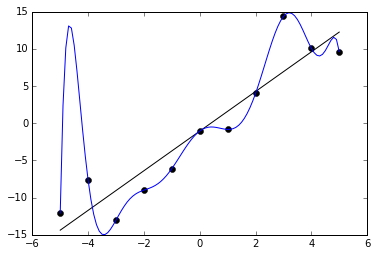
\includegraphics[width = 0.4\linewidth]{overfitting.png}}{\textcopyright \href{https://commons.wikimedia.org/wiki/File:Overfitted_Data.png}{Overfitted Data} by Ghiles, licensed under \href{https://creativecommons.org/licenses/by-sa/4.0}{CC BY-SA 4.0}, via Wikimedia Commons}
			\end{figure}
		\end{remark}

	\subsection{Probabilistic Interpretations}

		Let us jump away from regression for a moment and look at what happens if instead of trying to learn a function with inputs and outputs, we are instead trying to determine the parameters of some random variable given some datapoints drawn from it.

		To do this, suppose that any observation $z$ is drawn from the random variable $Z$ with probability density/mass function $g_\theta$ (depending on the parameter $\theta$, which we are trying to learn). For example, if $Z$ is a gaussian with mean $\mu$ and variance $\sigma^2$, we might have $\theta = (\mu,\sigma^2)$ and
		\[ g_\theta(z) = \frac{1}{\sigma\sqrt{2\pi}} \exp\left( -\frac{1}{2} \frac{(x-\mu)^2}{\sigma^2} \right). \]
	
		% Now, let us work w

		% Using an error function is not the only way to arrive at a good estimate of $w$. In fact, we need not even arrive at a single estimate of $w$, it might be better to finally arrive at some \emph{distribution} that represents how $w$ might behave depending on the information we have.\\

		\subsubsection{Maximum likelihood estimation}

			Suppose we are given a dataset $\mathcal{D} = \{z_1,\ldots,z_m\}$.\\
			Also suppose that we have discrete outputs for the moment ($g_w$ is a probability \emph{mass} function). Then, define the \emph{likelihood} function
			\[ \mathcal{L}(\mathcal{D} \mid \theta) = \Pr[ \mathcal{D} \mid \theta ]. \]
			Making the mild assumption that the various datapoints in $\mathcal{D}$ are drawn iid, this can be rewritten as
			\[ \mathcal{L}(\mathcal{D} \mid \theta) = \prod_{i=1}^m g_\theta(z_i). \]
			Even in the case where we have a continuous output (so a probability density function) instead, this expression remains the same.\\
			As might be expected, in \emph{maximum likelihood estimation} (MLE), we choose that $w$ which maximizes the likelihood. Often, we work with the \emph{log}-likelihood $\ell$ as well, which is just defined by $\ell(\mathcal{D} \mid w) = \log \mathcal{L}(\mathcal{D} \mid w)$.

		\subsubsection{Bayesian estimation}

			In all that we have done so far, we have arrived at a single estimate for $w$ or $\theta$. However, this may not necessarily be the best option -- might it not be better to arrive at a probability distribution for $w$ which represents how likely various values are?\\
			Bayesian estimation is one simple way of doing this.\\

			We make the assumption initially that $\theta$ is drawn from some \emph{prior} probability distribution $p$. Given the dataset $\mathcal{D} = \{z_1,\ldots,z_m\}$ (and the function $g_\theta$ from earlier), we try to improve on this prior to get to a \emph{posterior} probability distribution that better reflects how $\theta$ behaves, now that we have knowledge about the dataset. To do this, we use Bayes' law:

			\begin{align}
				\Pr[\theta\mid\mathcal{D}] &= \frac{\Pr[\mathcal{D}\mid\theta] \Pr[\theta]}{\Pr[\mathcal{D}]} \nonumber \\
					&= \frac{\Pr[\mathcal{D}\mid\theta] p(\theta)}{\int \Pr[\mathcal{D}\mid\alpha] p(\alpha) \dif \alpha}. \label{eqn: 1.1}
			\end{align}

			Note the contrast between this and MLE; in the the former we use $\Pr[\theta\mid\mathcal{D}]$, whereas in the latter we use $\Pr[\mathcal{D}\mid\theta]$.\\
			We can then use the posterior to return some estimate of $\theta$.\\
			In \emph{maximum a posteriori estimation} (MAP estimation), we return the mode of the posterior density.\\
			In \emph{Bayesian estimation}, we return the mean of the posterior density.\\
			In the pure Bayesian estimate, we do not return any point estimate for $\theta$ at all, and we instead use Bayes' rule to calculate the output given an input as
			\[ \Pr[x \mid \mathcal{D}] = \int p(x\mid\theta) p(\theta\mid\mathcal{D}) \dif \theta \]

			Now, the integral in the denominator of \eqref{eqn: 1.1} can be quite daunting. To deal with this, we introduce the idea of a \emph{conjugate prior}. Such a prior is of the form that the base distribution of both the prior and the posterior are the same. This then enables us to skip the calculation of the denominator, since it merely leads to a constant to normalize the distribution (its integral must be $1$), and we know this constant from the structure of the distribution anyway. This can be better understood by an example. Suppose that the datapoints are drawn from a Bernoulli distribution with parameter $\theta$. We then have
			\[ \Pr[\mathcal{D} \mid \theta] = \theta^r (1-\theta)^{m-r}, \]
			where $r$ is the number of $1$s in $\mathcal{D}$. If we choose our prior to be a \href{https://en.wikipedia.org/wiki/Beta_distribution}{Beta distribution} with parameters $\alpha$ and $\beta$, then the numerator of \eqref{eqn: 1.1} is
			\[ \theta^r (1-\theta)^{m-r} \cdot \theta^{\alpha-1} (1-\theta)^{\beta-1} \frac{\Gamma(\alpha)\Gamma(\beta)}{\Gamma(\alpha+\beta)}. \]
			This is proportional to $\theta^{\alpha+r-1}(1-\theta)^{m-r+\beta-1}$. Since the denominator only gives a constant multiplicative factor, the posterior must just be $\Beta(\alpha+r,\beta+m-r)$.\\

			Some more examples are that the \href{https://en.wikipedia.org/wiki/Dirichlet_distribution}{Dirichlet distribution} is the conjugate prior to the multivariate Bernoulli and the Gaussian is the conjugate prior to the Gaussian.

			% $y = w^\top \phi(x) + \varepsilon
			% \varepsilon \sim \mathcal{N}(0,\sigma^2)
			% w \sim \mathcal{N}(\mu_0,\Sigma_0)
			% \Sigma_m^{-1} = \Sigma_0^{-1} + \frac{1}{\sigma^2} \Phi^\top \Phi
			% \Sigma_m^{-1} \mu_m = \Sigma_0^{-1} \mu_0 + \Phi^\top y/\sigma^2$


			Bayesian estimation takes care of overfitting

		\subsubsection{Relating probabilistic interpretations and regression}

			Let us jump back to regression. While we typically assume that our input/output pairs are initially taken from some basic (fixed) function $f$, this is typically not the case. Indeed, we usually have some amount of error when taking the observations itself. This error is commonly taken to be a Gaussian with $0$ mean and some (small) variance $\sigma^2$.\\
			The output as a whole is then just a random variable, with the parameters involving our base parameter $\theta$ \emph{and} the input.\\
			
			For example, let our training data set be $\mathcal{D} = \{\langle x_1,y_1\rangle,\ldots,\langle x_m,y_m\rangle\}$ where the $x_i$ are in $\Rn$ and the $y_i$ in $\R$. Let us perform normal linear regression, but also add a Gaussian error of known variance $\sigma^2$. That is, if the input is $x$, we predict the distribution of the corresponding output $y$ to be $\mathcal{N}(w^\top x, \sigma^2)$.\\
			Supposing we use MLE, we wish to determine
			\[ \hat{w} = \argmax_{w} \frac{1}{(\sqrt{2\pi}\sigma)^m} \exp \left( -\frac{1}{2\sigma^2} \sum_{i=1}^m (y_i - w^\top x_i)^2 \right). \]
			It is not too difficult to see that this is in fact the same solution as that given by the discussion in \hyperref[subsubsec: the method of least squares]{the method of least squares}.

	\subsection{Regularisation}

		As mentioned in a remark towards the end of \Cref{subsubsec: the method of least squares}, overfitting tends to make the error over the test data too large, due to large fluctuations in the model we learn (to emulate the training data better). However, this also leads to large coefficients of the learnt vector, and thus large norm. Regularisation attempts to fix this, by further adding in the constraint that $\norm{w}_2$ is not too large.

		\subsubsection{Regularised regression}

			This leads to the \emph{penalized regularised least squares regression problem}, where the cost function is replaced with
			\[ \norm{\Phi w - y}_2^2 + \lambda\Omega(w). \]
			We are said to be performing
			\begin{itemize}
				\item \emph{ridge regression} if $\Omega(w) = \norm{w}_2^2$,
				\item \emph{lasso\footnote{this is an abbreviation for \emph{l}east \emph{a}bsolute \emph{s}hrinkage and \emph{s}election \emph{o}perator} regression} if $\Omega(w) = \norm{w}_1$, and
				\item \emph{support-based penalty regression} if $\Omega(w) = \norm{w}_0$.
			\end{itemize}
			The closed-form solutions to the first two can be computed by setting the gradient to $0$. In particular, the closed-form solution for ridge regression is
			\[ \hat{w} = (\Phi^\top\Phi + \lambda I)^{-1} \Phi^\top y. \]
			Also, this turns out to be the same as performing Bayes/MAP estimation with a multivariate Gaussian prior of mean $0$ and variance $(1/\lambda)I$.\\

			Alternatively, we have the \emph{constrained regularised least squares regression problem}, where the cost function is the normal $\norm{\Phi w - y}_2^2$, but we have the added constraint that $\Omega(w) \le \theta$ for some fixed $\theta$.\\
			We again have ridge, lasso, or support-based penalty regression depending on $\Omega$.\\
			It in fact turns out that the above two constraints are equivalent -- for any penalized formulation with a $\lambda$, there is a corresponding constrained formulation problem with some $\theta$ (that depends on both $\lambda$ and the data), and vice-versa.\\

			Why is lasso regression interesting? Observe that the level curves of $\norm{w}_1$ (namely cross-polytopes) have many corners on the axes, and as a result, it is likely that many components of $w$ are close to $0$ (as opposed to ridge regression where the level curves are rotationally invariant). That is, the learnt vector is likely very sparse, which is desirable.\\
			The closed form solution is the MAP estimate of linear regression subject to the prior being the \href{https://en.wikipedia.org/wiki/Laplace_distribution}{Laplace distribution} with parameters $0$ and $\theta$. Note that the Laplace distribution is extremely similar to the Gaussian, except that we use the $L^1$ norm in the exponential instead of the $L^2$. The intuition that lasso regression leads to many parameters being close to $0$ is strengthened by the sparsity of the Laplace distribution (the density at $0$ is high).\\
			However, there is no known closed form solution for the solution to lasso regression. Instead, it is solved iteratively with normal gradient descent. We have
			\begin{align*}
				\hat{w} &= \argmin_w \norm{\Phi w - y}_2^2 + \lambda\norm{w}_1 \\
					&= \argmin_w E_{\text{LS}}(w) + \lambda\norm{w}_1.
			\end{align*}
			At the $k$th step, set
			\begin{align*}
				w_{\text{LS}}^{k+1} &= w_{\text{Lasso}}^{k} - \eta\nabla E_\text{LS}(w_\text{Lasso}^{k}) \\
				(w_\text{Lasso}^{k+1})_{i} &=
				\begin{cases}
					(w_\text{LS}^{k+1})_i - \lambda\eta, & (w_\text{LS}^{k+1})_i > \lambda\eta, \\
					(w_\text{LS}^{k+1})_i + \lambda\eta, & (w_\text{LS}^{k+1})_i < -\lambda\eta, \\
					0, & \text{otherwise.}
				\end{cases}
			\end{align*}
			We then estimate $\hat{w}$ as $w_\text{Lasso}^r$ for a suitably large $r$.

		\subsubsection{Understanding regularisation}

			Ridge regression might seem slightly silly from the perspective of just training error. Indeed, the the (minimized) error for the ridge cost function is always greater than the (minimized) error for normal least squares.\\

			Suppose we are performing regression with a true function $g$ and let $f$ be our predicted/fitted function. We sample a bunch of points from $g$ to get a dataset, with possibly some noise that causes small perturbations.\\
			There are three primary sources of test error:
			\begin{itemize}
				\item \emph{Bias}: This occurs due to the difference between the nature of the true function and fitted function. It is just equal to $\expec[f(x)] - g(x)$.
				\item \emph{Variance}: This occurs due to the choice of our dataset. It is equal to $\Var(f(\hat{x}))$.
				\item \emph{Noise}: This occurs due to the implicit noise that is present when we take measurements from the true function. For example, there may be an additive Gaussian noise with mean $0$ and variance $\sigma^2$. The noise is then just equal to the variance $\sigma^2$ of this component.
			\end{itemize}

			Now, suppose the noise is some random variable $\varepsilon$ with mean $0$ and variance $\sigma^2$. Then, given an input $x$, we observe the output $y$ as being drawn from $g(x)+\varepsilon$.\\
			Suppose we are given a dataset $\mathcal{D} = \{\langle x_i,y_i\rangle : 1 \le i\le m\}$, and using it we predict the function $f$.\\
			The question we would like to answer is: what is the expected test error $\expec[(f(\hat{x}) - (g(\hat{x}) + \varepsilon))^2]$ for a new input $\hat{x}$? The expectation is taken over both the sampled dataset and the distribution of $\varepsilon$.\\
			Let $\hat{y} = g(\hat{x}) + \varepsilon$. We then have
			\begin{align*}
				\expec[(f(\hat{x}) - \hat{y})^2] &= \expec[f(\hat{x})^2] + \expec[\hat{y}^2] - 2 \expec[f(\hat{x})]\expec[\hat{y}] & \text{(assuming the dataset and $\varepsilon$ are independent)} \\
					&= \expec[f(\hat{x})]^2 + \Var(f(\hat{x})) + \expec[\hat{y}^2] - 2 \expec[\hat{f}(x)] g(\hat{x}) \\
					&= \expec[f(\hat{x})]^2 + \Var(f(\hat{x})) + \expec[g(\hat{x})^2 + \varepsilon^2] - 2 \expec[\hat{f}(x)] g(\hat{x}) \\
					&= \expec[f(\hat{x})]^2  + g(\hat{x})^2 - 2 \expec[\hat{f}(x)] g(\hat{x}) + \Var(f(\hat{x})) + \sigma^2 \\
					&= \underbrace{(\expec[f(\hat{x})] - g(\hat{x}))^2}_{\textstyle\text{Bias$^2$}} + \underbrace{\Var(f(\hat{x}))}_{\textstyle\text{Variance}} + \underbrace{\sigma^2 \mathstrut}_{\textstyle\text{Noise}}.
			\end{align*}

			Given the bias-variance tradeoff, how do we choose the best predictor? How do we set the model's parameters?\\
			In \emph{bootstrap sampling}, we repeatedly sample observations from a dataset with replacement. Given dataset $\mathcal{D}_b$, we repeatedly choose a $V_b$, train on $\mathcal{D}_b \setminus V_b$, then test on $V_b$.\\
			So, the training set is that we use to actually train the algorithm. $V_b$ is the \emph{validation} or \emph{development} set, and is used for model selection and tuning hyperparameters. The test/evaluation set is that we use for testing finally.

\section{Classification}

	Suppose we wish to intelligently classify emails into two categories depending on whether they are spam or not. How do we learn a method to classify an email as spam?

	It is not similar to regression where the function maps to $\R$, but we instead map to a discrete set $\{c_1,c_2,\ldots,c_k\}$.\\
	The simple hack of mapping $c_i$ to $i$, say, and then performing usual regression. However, the ordering of the $c_i$ influences it significantly then, which is very undesirable, since the ordering doesn't mean anything.\\
	A better idea would be to take $c_i$ as
	\[ y_i = e_i \in \R^k, \]
	to encode the idea that the various components are `independent'.\\
	We present these ideas over the next few sections.

	\subsection{Perceptron Classification}

		\subsubsection{The basic idea}

			Rather than mapping directly to $\mathcal{C} = \{c_1,\ldots,c_k\}$, we could map to some intermediate space which in turn maps to $\mathcal{C}$ (or a sequence of spaces and functions, the last of which is $\mathcal{C}$).\\

			First, consider the binary classification problem, where $\mathcal{C} = \{-1,1\}$. Let $\mathcal{D} = \{ \langle x_i , y_i \rangle : 1 \le i \le m \}$, where each $y_i \in \{-1,1\}$. The ordering does not matter then (both orderings are equivalent), so we can learn a linear classifier. Suppose $f(x) = w^\top \phi(x)$.\\
			Given a new input $x$, we predict the new output as $1$ if $f(x) \ge 0$ and $-1$ if $f(x) < 0$. So, we want
			\[ y\cdot w^\top \phi(x) \ge 0. \]

			We learn $w$ as follows. Starting with $w^{(0)} = 0$, we iterate over the dataset. If a point is correctly classified, we leave $w^{(r+1)} = w^{(r)}$. Otherwise, we marginally correct the weights by performing
			\[ w^{(r+1)} = w^{(r)} + \eta y_{r+1}\phi(x_{r+1}), \]
			for some (typically small) learning rate $\eta$.\\
			Observe that the quantity $w^\top \phi(x)$ is the distance of $x_r$ from the hyperplane $\{x : w^\top\phi(x) = 0\}$.\\
			So,
			\[ y_{r+1}(w^{(r+1)})^\top \phi(x_r) = y_{r+1} (w^{(r)})^\top\phi(x_{r+1}) + \eta\norm{\phi(x_{r+1})}^2. \]
			This makes the quantity $y_{r+1} w^\top \phi(x_r)$ less negative. We repeat the above process until $y_iw^\top\phi(x_i) \ge 0$ for all $i$ (or until we terminate). \\
			This \emph{perceptron} algorithm does not attempt to find the best separating hyperplane, it merely tries to find any separating hyperplane -- it need not provide any `breathing room' for the inputs. This is addressed by support vector machines, which we shall read later.\\
			One issue with perceptron classification is that it does not acknowledge how much the estimate differs from the expected $\pm 1$ -- we only care that $yw^\top\phi(x) \ge 0$, not how positive it is.

		\subsubsection{Convergence}

			Now, suppose there exists some $u$ such that for all $i$, $y_i u^\top \phi(x_i) \ge 0$. It turns out that the perceptron update rule will then converge in a finite number of iterations. That is, perceptrons can model linearly separable functions.
			\begin{proof}
				Since we can normalize $u$ suppose that $\norm{u} = 1$. We can also normalize the dataset itself, so assume $\norm{\phi(x_i)} \le 1$ for all $i$. \\
				Define the \emph{margin} $\gamma = \min_i |u^\top x_i|$.\\
				Further make the assumption that $\eta = 1$ (the general case follows similarly.) \\
				We claim that in at most $t = 1/\gamma^2$ updates, we will have $y_i {w^{(t)}}^\top x_i > 0$ for all $i$.\\
				If we update $w^{(k)}$ to $w^{(k+1)} = w^{(k)} + y\phi(x)$ on reading the input $\langle x,y\rangle$,
				\[ {w^{(k+1)}}^\top u =  (w^{(k)}+y\phi(x))^\top u \ge {w^{(k)}}^\top u + \gamma. \]
				and
				\[ \norm{w^{(k+1)}}^2 = \norm{w^{(k)} + y\phi(x)}^2 < \norm{w^{(k)}}^2 + 1. \]
				As a result, after $k$ updates,
				\[ {w^{(k)}}^\top u \ge k\gamma \text{ and } \norm{w^{(k)}}^2 \le k \]
				so
				\[ \sqrt{k} \ge \underbrace{\norm{w^{(k)}} \ge u^\top w^{(k)}}_{\text{Using Cauchy-Schwarz}} \ge k\gamma. \]
				This gives $k \le 1/\gamma^2$, completing the proof.
			\end{proof}

		\subsubsection{Viewing the algorithm with a loss function}

			Consider the loss function
			\[ L_P(w^\top(\phi(x)),y) = \max\{ 0 , -yw^\top\phi(x) \}. \]
			We can then apply the \emph{stochastic gradient descent} algorithm. Let $f_w(x) = w^\top\phi(x)$ and choose some example $\langle x_t,y_t\rangle$. We then compute the gradient of the loss of $f_w(x_t)$ with respect to $w$, then update the weight vector using it as
			\[ w \gets w - \nabla_w L_P(f_w(x_t),y). \]
			Perceptron update is then just stochastic gradient descent on this ``hinge loss'' function.\\
			Similarly, we could use different loss functions.\\

			Now, what $w$ should we use at the time of testing? Using the final $w$ is not always a good idea due to overfitting and the stochastic nature of the algorithm.\\
			So, we usually use an intermediate $w$. The \emph{voted perceptron} algorithm counts votes for weight vectors tallying how many examples they have correctly classified. The \emph{averaged perceptron} algorithm uses the averaged weight vector (not necessarily the average of all weight vectors, but a suitable subset).\\

			Typically, rather than doing stochastic gradient descent datapoint by datapoint, we evaluate it in batches datapoint. That is, we do
			\[ w \gets w - \frac{1}{|\mathcal{B}|} \sum_{(x,y) \in \mathcal{B}} \nabla_w L_P(f_w(x),y) \]
			for a suitable batch $B$, which is intermediate between normal gradient descent and stochastic gradient descent. Observe that if $B$ is the entire dataset, we get ordinary gradient descent.

	\subsection{Logistic Regression}

		Recall that the function we use in perceptron classification is just a step function. Is it possible to do better, and possibly take care of smoothness issues? That is, instead of $\operatorname{sign}(w^\top\phi(x))$, can we use some more general $\Omega(w^\top \phi(x))$? In logistic regression, we use the \textit{sigmoid function} defined by
		\[ \sigma(t) = \frac{1}{1+e^{-t}}. \]
		Rather than looking at whether the value of the function is positive or negative, we instead see here whether it is greater than or less than $1/2$. Now, let us return to the binary classification problem, taking $\mathcal{C} = \{0,1\}$ instead of $\{-1,1\}$. Since the sigmoid maps into $(0,1)$, this also allows us a probabilistic interpretation as
		\[ \Pr[y=1 \mid x] = \frac{1}{1+e^{-w^\top \phi(x)}} \text{ and } \Pr[y=0\mid x] = \frac{e^{-w^\top \phi(x)}}{1+e^{-w^\top \phi(x)}}. \]
		That is, we can view it as a Bernoulli model with parameter $\sigma(w^\top\phi(x))$.\\
		We can then do maximum likelihood estimation for the parameter of the Bernoulli (or minimize the error), and thus arrive at an estimate for $w$! We can also do something along the lines of Bayesian or MAP estimation.\\
		To be more explicit, the maximum likelihood estimate is is
		\begin{align*}
			\hat{w} &= \argmax_w \mathcal{L}(\mathcal{D};w) \\
				&= \argmax_w \Pr\left[ y_1,\ldots,y_m \mid w,x_1,\ldots,x_m \right] \\
				&= \argmax_w \prod_{i=1}^m \Pr\left[ y_i \mid w, x_i \right] \\
				&= \argmax_w \prod_{i=1}^m \sigma(w^\top\phi(x_i))^{y_i} (1 - \sigma(w^\top\phi(x_i)))^{1-y_i} \\
				&= \argmax_w \sum_{i=1}^m y_i \log(w^\top \phi(x_i)) + (1 - y_i) \log(1-\sigma(w^\top\phi(x_i))) \\
				&= \argmin_w \underbrace{- \sum_{i=1}^m y_i \log(w^\top \phi(x_i)) + (1 - y_i) \log(1-\sigma(w^\top\phi(x_i)))}_{-\log(\mathcal{L}(\mathcal{D};w))}.
		\end{align*}
		The average negative log-likelihood ($- 1/m \log(\mathcal{L}(\mathcal{D};w))$) is often referred to as the \emph{cross-entropy} loss function $E(w)$, and represents a ``distance'' between the data distribution (the $y_i$) and the model distribution (the $\sigma$). Cross-entropy is the average number of bits required to identify an event drawn from the dataset, if a coding scheme is used that is optimized for a modelled probability distribution $\Pr[y\mid\mathcal{M}]$ (as opposed to the `true' distribution $\Pr[y\mid\mathcal{D}]$).\\
		Alternatively, we have
		\[ E(w) = - \frac{1}{m} \sum_{i=1}^m y_i w^\top \phi(x_i) - \log(1 + e^{w^\top\phi(x_i)}). \]
		The first component here resembles the loss in perceptron classification.\\
		We do not have a simple closed-form solution for the cross-entropy loss function, so we apply gradient descent. The update rule looks like
		\[ w^{(k+1)} = w^{(k)} + \eta \left(\frac{1}{m} \sum_{i=1}^m (y_i - \sigma({w^{(k)}}^\top\phi(x_i))) \phi(x_i) \right). \]
		The stochastic version of this is
		\[ w^{(k+1)} = w^{(k)} + \eta (y_i - \sigma({w^{(k)}}^\top\phi(x_i))) \phi(x_i). \]
		We shall return to something similar when we study generalized linear models later in the course, of which perceptron, linear regression, and logistic regression are special cases.\\
		The \emph{regularized} (logistic) cross-entropy loss function is
		\[ E_r(w) = -\frac{1}{m} \sum_{i=1}^m y_i \log(w^\top \phi(x_i)) + (1 - y_i) \log(1-\sigma(w^\top\phi(x_i))) + \frac{\lambda}{2m}\norm{w}_2^2, \]
		which attempts to avoid overfitting. The probabilistic interpretation of this is that this is the MAP estimate given a Gaussian prior on $w$ with mean $0$ and variance $1/\lambda$. In this case, the gradient descent update rule is
		\[ w^{(k+1)} = w^{(k)} + \eta \left(\frac{1}{m} \sum_{i=1}^m (y_i - \sigma({w^{(k)}}^\top\phi(x_i))) \phi(x_i) - \lambda w^{(k)} \right). \]

		Logistic regression is easily extended to even the multi-class scenario (say $k$ classes $1,\ldots,k$), by keeping a different weight vector $w_{c}$ for each $1\le c\le k-1$, then letting
		\[ \Pr[y=c\mid x] = \frac{e^{-w_c^\top \phi(x)}}{1 + \sum_{i=1}^{k-1} e^{-w_i^\top \phi(x)}} \]
		for $1\le c\le k-1$ and
		\[ \Pr[y=k\mid x] = \frac{1}{1 + \sum_{i=1}^{k-1} e^{-w_i^\top \phi(x)}}. \]
		We can have parameters for all $k$ classes, but this is not necessary since the $k$th class occurs iff none of the other $k-1$ classes occurs.

% \bibliographystyle{alpha}
% \bibliography{references}


\end{document}